% questions.tex —— 2002 年·全国旧课程卷·文科 · 题目内容片段（无答案）
% 由 tools/generate_projects.py 依来源总账自 2002/2002_数学真题_全国旧课程文_试题.md 生成，勿手改（改源 MD 后重跑）


\gkpart{数学}

\begin{gktip}
\textbf{来源说明}：本题面依据固定源 PDF 两页 A3 题面逐题转录，原卷印刷页码 106–107。固定源不附答案，答案和解析均由本库独立复算。

\textbf{图形说明}：第 13、17、19、22 题的原卷图形关系重绘为 TikZ/PGFPlots 矢量图。图形标记所指的 PNG 不随仓库保存。
\end{gktip}

\gkpart{一、选择题}

\begin{question}
\gkti{1}直线 $(1+a)x+y+1=0$ 与圆 $x^2+y^2-2x=0$ 相切，则 $a$ 的值为\mbox{（　　）}

（A）$\pm1$　　（B）$\pm2$　　（C）$1$　　（D）$-1$

\end{question}
\begin{question}
\gkti{2}复数

\nopagebreak[4]
\[
\left(\frac12+\frac{\sqrt3}{2}i\right)^3
\]

的值是\mbox{（　　）}

（A）$-i$　　（B）$i$　　（C）$-1$　　（D）$1$

\end{question}
\begin{question}
\gkti{3}不等式 $(1+x)(1-|x|)>0$ 的解集是\mbox{（　　）}

（A）$\{x\mid 0\leqslant x<1\}$

（B）$\{x\mid x<0\text{ \text{且} }x\neq-1\}$

（C）$\{x\mid -1<x<1\}$

（D）$\{x\mid x<1\text{ \text{且} }x\neq-1\}$

\end{question}
\begin{question}
\gkti{4}函数 $y=a^x$ 在 $[0,1]$ 上的最大值与最小值之和为 $3$，则 $a=$\mbox{（　　）}

（A）$\frac12$　　（B）$2$　　（C）$4$　　（D）$\frac14$

\end{question}
\begin{question}
\gkti{5}在 $(0,2\pi)$ 内，使 $\sin x>\cos x$ 成立的 $x$ 的取值范围是\mbox{（　　）}

（A）$\left(\frac\pi4,\frac\pi2\right)\cup\left(\pi,\frac{5\pi}4\right)$

（B）$\left(\frac\pi4,\pi\right)$

（C）$\left(\frac\pi4,\frac{5\pi}4\right)$

（D）$\left(\frac\pi4,\pi\right)\cup\left(\frac{5\pi}4,\frac{3\pi}2\right)$

\end{question}
\begin{question}
\gkti{6}设集合

\nopagebreak[4]
\[
M=\left\{x\middle|x=\frac{k}{2}+\frac14,\ k\in\mathbb Z\right\},\qquad
N=\left\{x\middle|x=\frac{k}{4}+\frac12,\ k\in\mathbb Z\right\},
\]

则\mbox{（　　）}

（A）$M=N$　　（B）$M\subseteq N$　　（C）$M\supseteq N$　　（D）$M\cap N=\varnothing$

\end{question}
\begin{question}
\gkti{7}椭圆 $5x^2+ky^2=5$ 的一个焦点是 $(0,2)$，那么 $k=$\mbox{（　　）}

（A）$-1$　　（B）$1$　　（C）$\sqrt5$　　（D）$-\sqrt5$

\end{question}
\begin{question}
\gkti{8}一个圆锥和一个半球有公共底面，如果圆锥的体积恰好与半球的体积相等，那么这个圆锥轴截面顶角的余弦值是\mbox{（　　）}

（A）$\frac34$　　（B）$\frac45$　　（C）$\frac35$　　（D）$-\frac35$

\end{question}
\begin{question}
\gkti{9}已知 $0<x<y<a<1$，则有\mbox{（　　）}

（A）$\log_a(xy)<0$

（B）$0<\log_a(xy)<1$

（C）$1<\log_a(xy)<2$

（D）$\log_a(xy)>2$

\end{question}
\begin{question}
\gkti{10}函数 $y=x^2+bx+c$，$x\in[0,+\infty)$ 是单调函数的充要条件是\mbox{（　　）}

（A）$b\geqslant0$　　（B）$b\leqslant0$　　（C）$b>0$　　（D）$b<0$

\end{question}
\begin{question}
\gkti{11}设 $\theta\in\left(0,\dfrac\pi4\right)$，则二次曲线

\nopagebreak[4]
\[
x^2\cot\theta-y^2\tan\theta=1
\]

的离心率的取值范围为\mbox{（　　）}

（A）$\left(0,\frac12\right)$　　（B）$\left(\frac12,\frac{\sqrt2}{2}\right)$

（C）$\left(\frac{\sqrt2}{2},2\right)$　　（D）$(\sqrt2,+\infty)$

\end{question}
\begin{question}
\gkti{12}从正方体的 6 个面中选取 3 个面，其中有 2 个面不相邻的选法共有\mbox{（　　）}

（A）8 种　　（B）12 种　　（C）16 种　　（D）20 种

\end{question}
\gkpart{二、填空题}

\Needspace{0.4\textheight}
\begin{question}
\gkti{13}据新华社 2002 年 3 月 12 日电，1985 年到 2000 年间，我国农村人均居住面积如图所示，其中，从\gkblank{}年到\gkblank{}年的五年间增长最快。
\nopagebreak[4]
\begin{center}% 2002 年全国旧课程文科第 13 题：农村人均居住面积柱状图
\begin{tikzpicture}[x=0.85cm,y=0.22cm,>=stealth]
  \draw[->] (0,0)--(5.4,0) node[right] {年份};
  \draw[->] (0,0)--(0,29) node[above] {面积/$\mathrm{m^2}$};
  \foreach \y/\label in {10/10,15/15,20/20,25/25}
    \draw (-0.12,\y)--(0.12,\y) node[left=5pt] {\label};
  \foreach \x/\label in {1/1985,2.3/1990,3.6/1995,4.9/2000}
    \draw (\x,0.15)--(\x,-0.15) node[below=4pt] {\label};
  \foreach \x/\h/\label in {
    1/14.7/14.7,
    2.3/17.8/17.8,
    3.6/21.0/21.0,
    4.9/24.8/24.8}
  {
    \draw[fill=gray!25] (\x-0.32,0) rectangle (\x+0.32,\h);
    \node[above=3pt] at (\x,\h) {\label};
  }
\end{tikzpicture}
\end{center}
\nopagebreak[4]
\begin{center}
\begin{tabular}{lrrrr}
\toprule
年份 & 1985 & 1990 & 1995 & 2000 \\
\midrule
人均居住面积（$\mathrm{m^2}$） & 14.7 & 17.8 & 21.0 & 24.8 \\
\bottomrule
\end{tabular}
\end{center}

\end{question}
\begin{question}
\gkti{14}函数

\nopagebreak[4]
\[
y=\frac{2x}{1+x},\qquad x\in(-1,+\infty)
\]

图象与其反函数图象的交点为\gkblank{}。

\end{question}
\begin{question}
\gkti{15}$(x^2+1)(x-2)^7$ 展开式中 $x^3$ 的系数是\gkblank{}。

\end{question}
\begin{question}
\gkti{16}对于顶点在原点的抛物线，给出下列条件：

① 焦点在 $y$ 轴上；

② 焦点在 $x$ 轴上；

③ 抛物线上横坐标为 $1$ 的点到焦点的距离等于 $6$；

④ 抛物线的通径的长为 $5$；

⑤ 由原点向过焦点的某条直线作垂线，垂足坐标为 $(2,1)$。

能使这抛物线方程为 $y^2=10x$ 的条件是\gkblank{}。（要求填写合适条件的序号）

\end{question}
\gkpart{三、解答题}

\Needspace{0.4\textheight}
\begin{question}
\gkti{17}如图，某地一天从 6 时至 14 时的温度变化曲线近似满足函数

\nopagebreak[4]
\[
y=A\sin(\omega x+\varphi)+b.
\]
\nopagebreak[4]
\begin{center}% 2002 年全国旧课程文科第 17 题：温度变化曲线
\begin{tikzpicture}[x=0.62cm,y=0.13cm,>=stealth]
  \draw[->] (5.2,0)--(14.8,0) node[right] {$t/\mathrm h$};
  \draw[->] (5.2,0)--(5.2,34) node[above] {$T/{}^\circ\mathrm C$};
  \foreach \y in {10,20,30}
    \draw[dashed,gray] (5.2,\y)--(14,\y) node[right] {\y};
  \foreach \x in {6,8,10,12,14}
    \draw (\x,0.4)--(\x,-0.4) node[below=3pt] {\x};
  \draw[thick,domain=6:14,samples=80]
    plot (\x,{20+10*sin(22.5*(\x-10))});
  \node[below left] at (5.2,0) {$O$};
\end{tikzpicture}
\end{center}
\nopagebreak[4]
（1） 求这段时间的最大温差；

（2） 写出这段时间的函数解析式。

\end{question}
\begin{question}
\gkti{18}甲、乙物体分别从相距 70 米的两处同时相向运动。甲第 1 分钟走 2 米，以后每分钟比前 1 分钟多走 1 米，乙每分钟走 5 米。

（1） 甲、乙开始运动后几分钟相遇？

（2） 如果甲、乙到达对方起点后立即折返，甲继续每分钟比前 1 分钟多走 1 米，乙继续每分钟走 5 米，那么开始运动几分钟后第二相遇？

\Needspace{0.4\textheight}
\end{question}
\begin{question}
\gkti{19}四棱锥 $P-ABCD$ 的底面是边长为 $a$ 的正方形，$PB\perp$ 平面 $ABCD$。
\nopagebreak[4]
\begin{center}% 2002 年全国旧课程文科第 19 题：四棱锥 P-ABCD
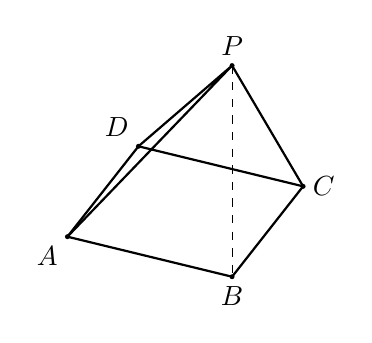
\begin{tikzpicture}[>=stealth,scale=0.82]
  \coordinate (A) at (0,0);
  \coordinate (B) at (2.55,-0.62);
  \coordinate (C) at (3.65,0.78);
  \coordinate (D) at (1.10,1.40);
  \coordinate (P) at (2.55,2.65);
  \draw[thick] (A)--(B)--(C)--(D)--cycle;
  \draw[thick] (P)--(A) (P)--(C) (P)--(D);
  \draw[dashed] (P)--(B);
  \fill (A) circle (1.1pt) node[below left] {$A$};
  \fill (B) circle (1.1pt) node[below] {$B$};
  \fill (C) circle (1.1pt) node[right] {$C$};
  \fill (D) circle (1.1pt) node[above left] {$D$};
  \fill (P) circle (1.1pt) node[above] {$P$};
\end{tikzpicture}
\end{center}
\nopagebreak[4]
（1） 若面 $PAD$ 与面 $ABCD$ 所成的二面角为 $60^\circ$，求这个四棱锥的体积；

（2） 证明无论四棱锥的高怎样变化，面 $PAD$ 与面 $PCD$ 所成的二面角恒大于 $90^\circ$。

\end{question}
\begin{question}
\gkti{20}设函数

\nopagebreak[4]
\[
f(x)=x^2+|x-2|-1,\qquad x\in\mathbb R.
\]

（1） 判断 $f(x)$ 的奇偶性；

（2） 求函数 $f(x)$ 的最小值。

\end{question}
\begin{question}
\gkti{21}已知点 $P$ 到两定点 $M(-1,0)\text{、}N(1,0)$ 距离的比为 $\sqrt2$，点 $N$ 到直线 $PM$ 的距离为 $1$，求直线 $PN$ 的方程。

\Needspace{0.4\textheight}
\end{question}
\begin{question}
\gkti{22}

（1） 给出两块相同的正三角形纸片（如图 1、图 2），要求用其中一块剪拼成一个三棱锥模型，另一块剪拼成一个正三棱柱模型，使它们的全面积都与原三角形的面积相等。请设计一种剪拼方法，分别用虚线标示在图 1、图 2 中，并作简要说明；

（2） 试比较你剪拼的正三棱锥与正三棱柱的体积大小；

（3） 如果给出的是一块任意三角形的纸片（如图 3），要求剪拼成一个直三棱柱，使它的全面积与给出的三角形的面积相等。请设计一种剪拼方法，用虚线标示在图 3 中，并作简要说明。
\nopagebreak[4]
\begin{center}% 2002 年全国旧课程文科第 22 题：剪拼示意
\begin{tikzpicture}[>=stealth,scale=0.76]
  % 图 1：沿三条中位线折成正四面体
  \begin{scope}[shift={(0,0)}]
    \coordinate (A) at (0,0);
    \coordinate (B) at (2.7,0);
    \coordinate (C) at (1.35,2.34);
    \coordinate (D) at ($(A)!0.5!(B)$);
    \coordinate (E) at ($(B)!0.5!(C)$);
    \coordinate (F) at ($(C)!0.5!(A)$);
    \draw[thick] (A)--(B)--(C)--cycle;
    \draw[dashed] (D)--(E)--(F)--cycle;
    \node at (1.35,-0.45) {图1};
  \end{scope}
  % 图 2：角部四边形剪下，余下部分折成缺上底的棱柱
  \begin{scope}[shift={(3.45,0)}]
    \coordinate (A) at (0,0);
    \coordinate (B) at (2.7,0);
    \coordinate (C) at (1.35,2.34);
    \coordinate (D) at ($(A)!0.5!(B)$);
    \coordinate (E) at ($(B)!0.5!(C)$);
    \coordinate (F) at ($(C)!0.5!(A)$);
    \draw[thick] (A)--(B)--(C)--cycle;
    \draw[dashed] (D)--(E)--(F)--cycle;
    \draw[dashed] (A)--(D) (B)--(E) (C)--(F);
    \node at (1.35,-0.45) {图2};
  \end{scope}
  % 图 3：任意三角形，内心和三条中点线
  \begin{scope}[shift={(6.9,0)}]
    \coordinate (A) at (0,0);
    \coordinate (B) at (2.95,0.15);
    \coordinate (C) at (1.0,2.25);
    \coordinate (I) at (1.25,0.82);
    \coordinate (D) at ($(I)!0.5!(A)$);
    \coordinate (E) at ($(I)!0.5!(B)$);
    \coordinate (F) at ($(I)!0.5!(C)$);
    \draw[thick] (A)--(B)--(C)--cycle;
    \draw[dashed] (I)--(A) (I)--(B) (I)--(C);
    \draw[dashed] (D)--(E)--(F)--cycle;
    \draw[dashed] (D)--($(D |- A)$) (E)--($(E |- B)$);
    \node at (1.35,-0.45) {图3};
  \end{scope}
\end{tikzpicture}
\end{center}
\nopagebreak[4]

\end{question}